\documentclass{article}
\usepackage[utf8]{inputenc}
\usepackage{amsmath}
\usepackage{mathtools}
\usepackage{relsize}
\usepackage{graphicx}
\graphicspath{ {./drift/} }
\DeclarePairedDelimiter{\ceil}{\lceil}{\rceil}
\usepackage{geometry}
\usepackage[banglamainfont=Kalpurush, 
            banglattfont=Siyam Rupali
           ]{latexbangla}
        
\begin{document}
\begin{LARGE}
\begin{center}
তাড়ন বেগ ও তড়িৎপ্রবাহ ঘনত্ব
\end{center}
\end{LARGE}
\textbf{গতিশীল তড়িৎচ্চালক বল:} ধরা যাক,  $ l $ দৈর্ঘ্যের একটি পরিবাহী একটি সুষম চৌম্বকক্ষেত্রে গতিশীল। চিত্রানুযায়ী  চৌম্বকক্ষেত্রের দিক পৃষ্ঠ থেকে বাইরের দিকে। পরিবাহীর অভ্যন্তরে থাকা $ q>0 $ চার্জ যুক্ত কণাগুলো একটি চৌম্বক বল $ \vec{F_{B}} = q\vec{v}\times \vec{B} $ অনুভব করে যা তাদেরকে পরিবাহীর উপরের দিকে এবং ঋনাত্নক চার্জগুলোকে পরিবাহীর উপরের নিচের দিকে ধাবিত করে। \\

\begin{center}
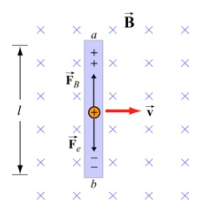
\includegraphics{2018-08-03_152836.png}
\end{center}


চার্জগুলোর এই বিভাজনের জন্য পরিবাহীর ভিতরে একটি বৈদ্যুতিক ক্ষেত্র $ \vec{E} $ উদ্ভব হয় যা একটি নিন্মমুখী বৈদ্যুতিক বল $ \vec{F} = q\vec{E} $ উৎপন্ন করে। সাম্যবস্থায় এই $ F_{B} $ এবং $ F_{E} $ একে অপরকে নিষ্ক্রিয় করে দেয় এবং পরিবাহীটির দুই প্রান্তে একটি বিভব পার্থক্য সৃষ্টি হয়।

\[V_{ab} = V_{a}-V_{b} = \varepsilon = El=Blv\]


যেহেতু পরিবাহীটির গতিশীলতার কারণে $ \varepsilon $ উদ্ভব হয় সেহেতু এই বিভব পার্থক্যকে বলা হয় গতিশীল তড়িচ্চালক বল।\\

এখন মনে করা যাক পরিবাহীটি একটি সুষম চৌম্বকক্ষেত্র $ \vec{B} = -B\hat{k} $ এর ভেতর দুটি ঘর্ষণহীন পরিবাহী পাতের উপর গতিশীল যারা $ w $ দুরত্বে অবস্থিত এবং একটি রোধ $ R $ দ্বারা সংযুক্ত।
\begin{center}
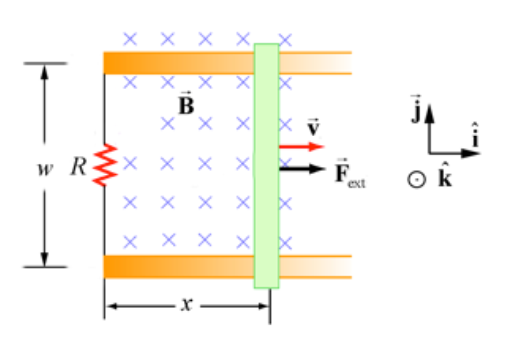
\includegraphics[width=0.5\textwidth]{2018-08-03_152853.png}
\end{center}

ধরা যাক, বাইরে থেকে একটি বল $ F_{ext} $ এমনভাবে প্রয়োগ করা হলো যা পরিবাহীটিকে $ \vec{v} = v\hat{i}$ সুষম বেগে গতিশীল করে। গতিশীল পরিবাহী এবং পাতদুটি দ্বারা একটি আবদ্ধ ক্ষেত্র $ \vec{A} = A\hat{k} $ বিবেচনা করা যাক যাক যার ভেতর দিয়ে গমনকারী চৌম্বক ফ্লাক্সের পরিমাণ,
\[\phi_{B} = \vec{B}\cdot \vec{A} = (-B\hat{k})\cdot (A\hat{k}) = -BA=-Bwx\]
তাহলে সময়ের সাপেক্ষে পরিবর্তনশীল চৌম্বকফ্লাক্স হবে,
\[ \dfrac{d}{dt}(\phi_{B}) = -\dfrac{d}{dt}(Bwx) = -Bw\dfrac{dx}{dt}=-Bwv\]
যেখানে, $ \dfrac{dx}{dt} = v $ হলো পরিবাহী বারটির বেগ। পরিবাহীর অভ্যন্তরে $ q $ চার্জযুক্ত একটি চার্জিত কণা একটি চৌম্বকবল অনুভব করবে যা, 
\[F_{B} = q\vec{v}\times\vec{B} = qv\hat{i}\times B(-\hat{k})= qvB\hat{j}\]

\end{document}